\section{Problem Description and Goals}

\begin{frame}
    \frametitle{Abstract}
    Text-based games, also called text adventures or interactive
    fiction, are a form of parser-driven text-based worlds where players
    control a Player Character in an immersive environment. Players
    interact with the environment by issuing text commands such as, ``go
    west'' or ``unlock the door with the bronze key'' and the game gives
    feedback in the form of natural language scene descriptions, e.g.
    ``You are standing in an open field west of a white house, with a
    boarded front door'' (Zork, Infocom, 1981). I would like to use
    pre-trained GloVe word embeddings to aid in parsing scene
    descriptions and action exploration, and, which in turn will be used
    to train a knowledge base that will be used for goal completion,
    with the hope that this will allow for effective knowledge transfer
    between a wide array of text adventure games.
\end{frame}

\begin{frame}[b]
    \begin{figure}
        \centering
        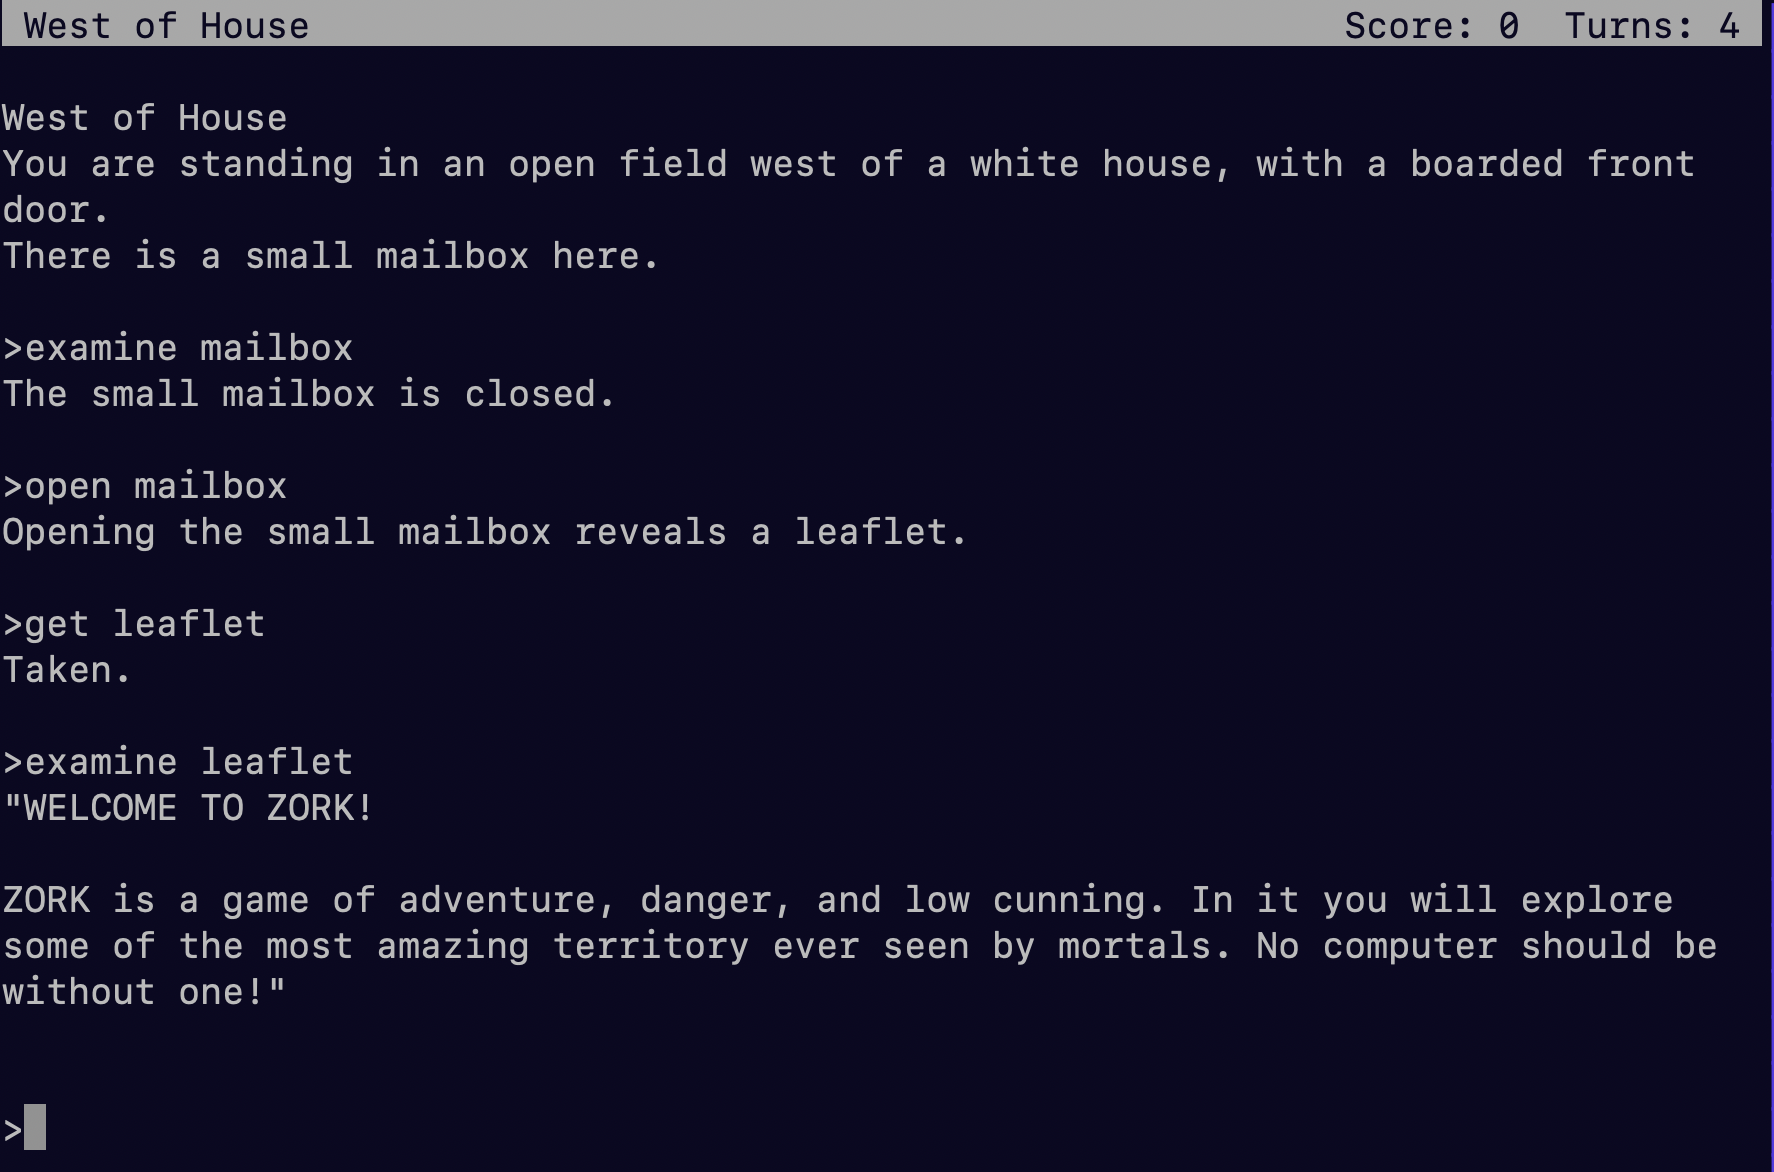
\includegraphics[width=\textwidth,keepaspectratio]{../images/zork1.png}
        \caption*{Zork I, Marc Blank and Dave Lebling, 1980}
    \end{figure}
\end{frame}

\begin{frame}[b]
    \begin{figure}
        \centering
        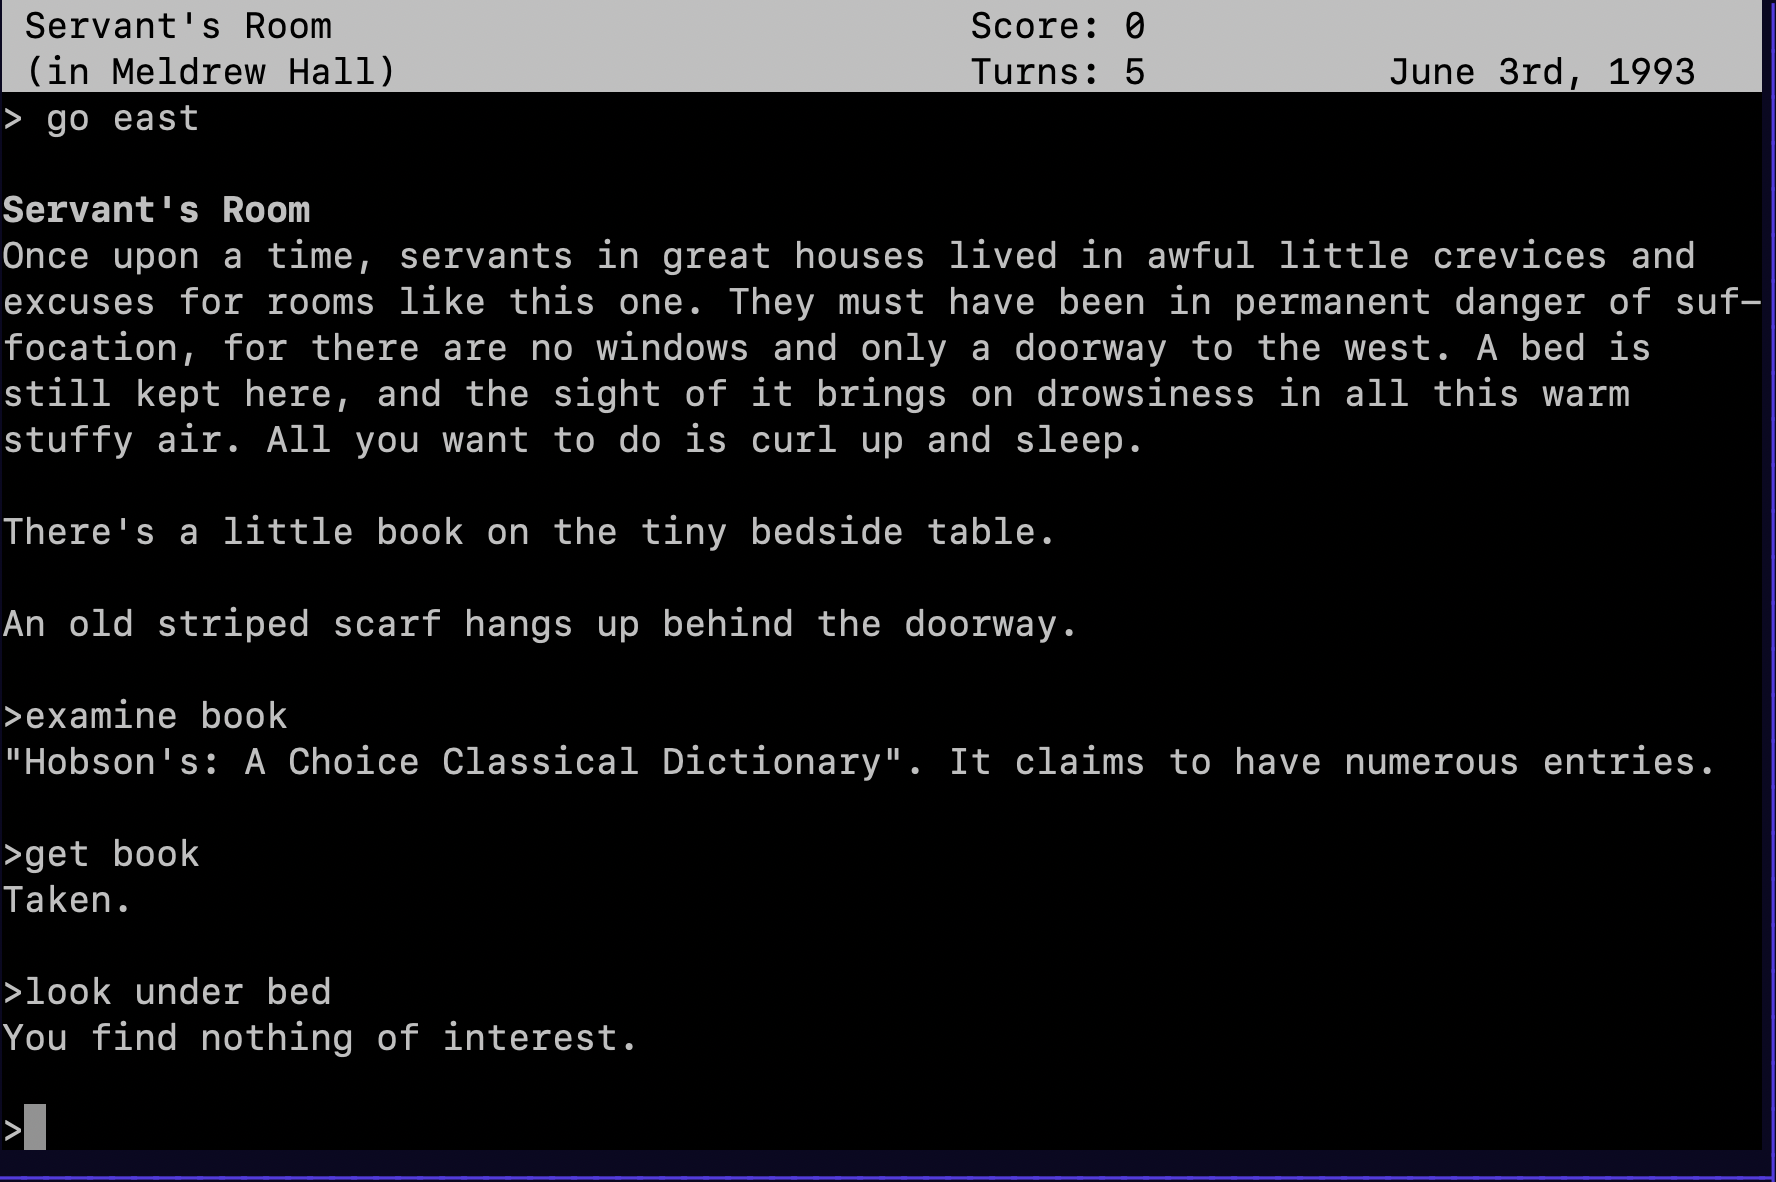
\includegraphics[width=\textwidth,keepaspectratio]{../images/curses.png}
        \caption*{Curses, Graham Nelson, 1993}
    \end{figure}
\end{frame}

\begin{frame}[b]
    \begin{figure}
        \centering
        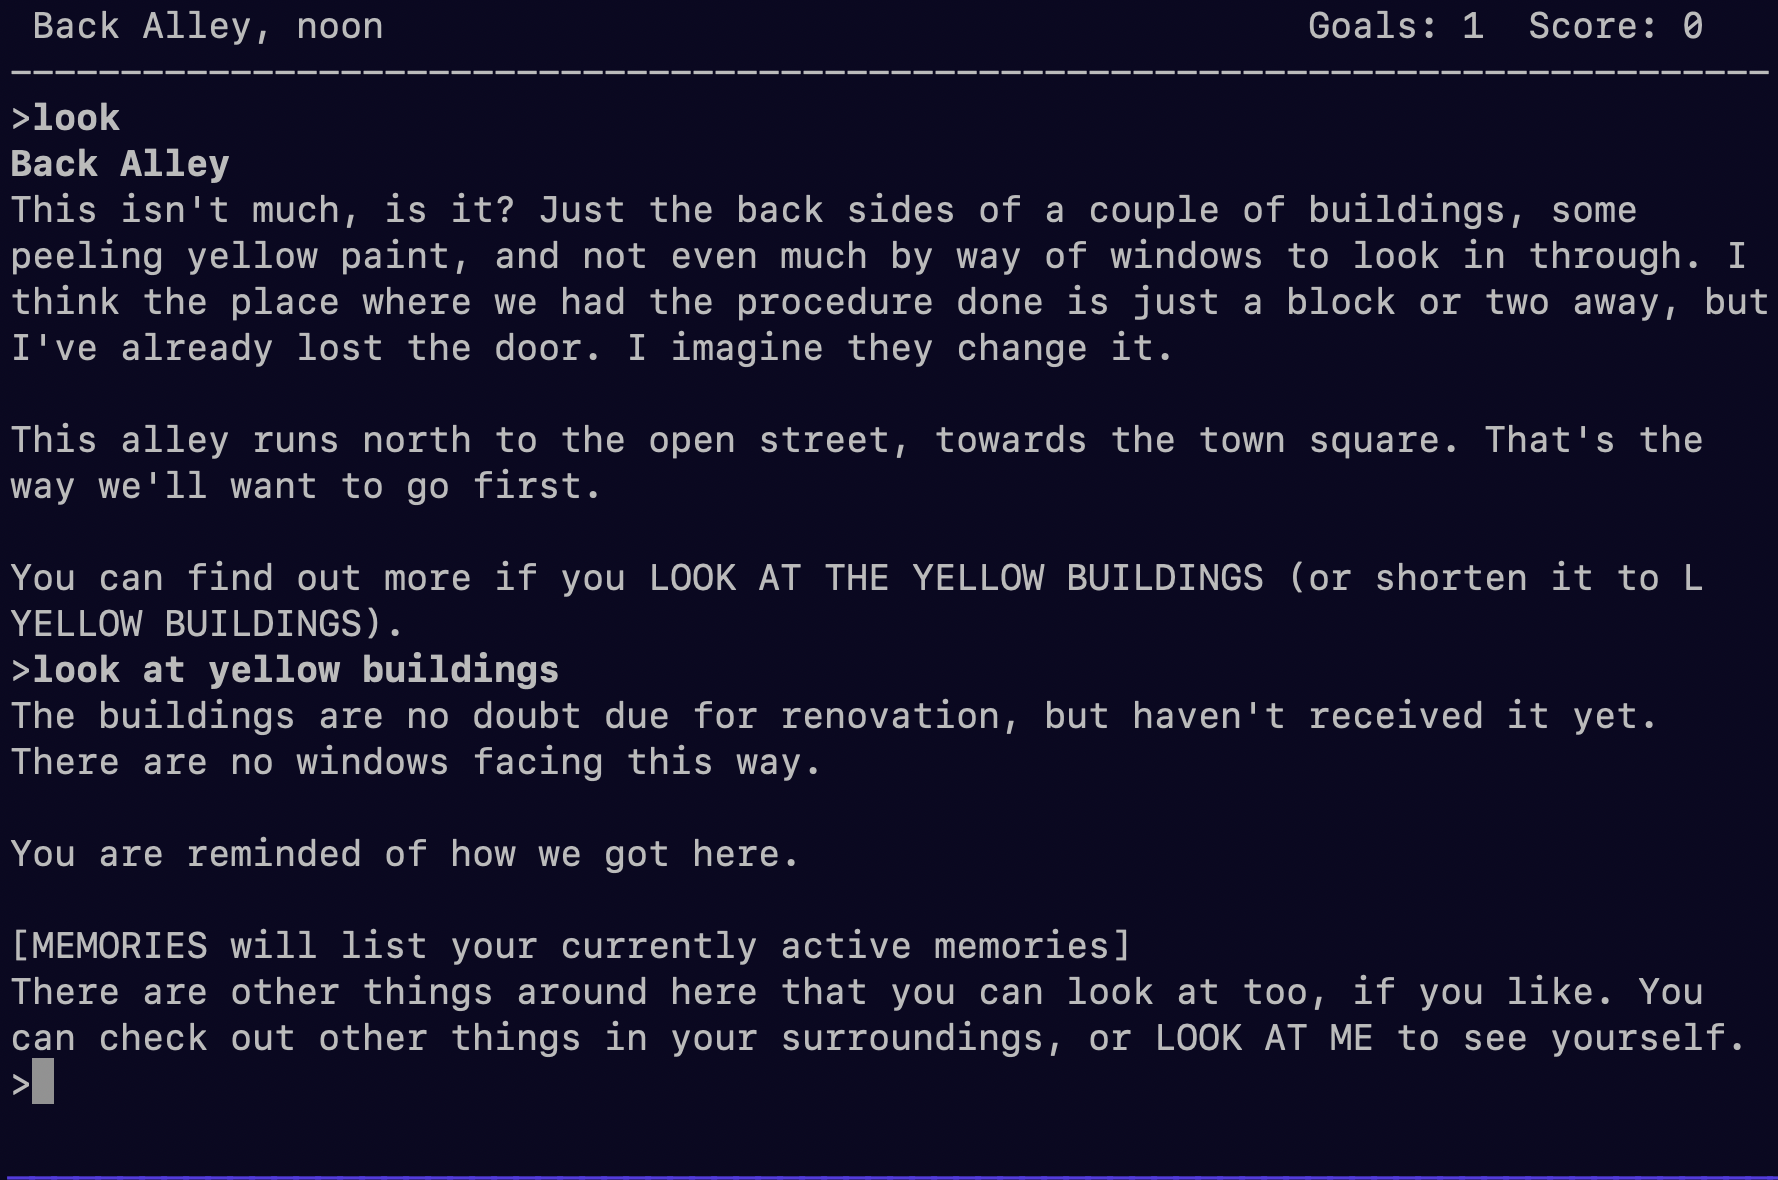
\includegraphics[width=\textwidth,keepaspectratio]{../images/counterfeit_monkey.png}
        \caption*{Counterfeit Monkey, Emily Short, 2012}
    \end{figure}
\end{frame}

\begin{frame}

    \frametitle{Text adventure games}
    \begin{columns}
    % timeline of popular games
        \column{.5\textwidth}
        \begin{block}{Popular games}
            {\footnotesize
            \begin{itemize}
                \item \game{Adventure}, William Crowther and Donald
                    Woods, 1976.
                \item \game{Zork I}, Mark Blank and Dave Lebling, 1980.
                \item \game{Enchanted}, Mark Blank and Dave Lebling,
                    1983.
                \item \game{The Hitchiker's Guide to the Galaxy},
                    Douglas Adams and Steve Meretsky, 1984.
                \item \game{Curses}, Graham Nelson, 1993.
                \item \game{Spider and Web}, Andrew Plotkin, 1998.
                \item \game{Counterfeit Monkey}, Emily Short, 2012.
            \end{itemize}
            \parencite{interactive_fiction_technology_foundation_interactive_nodate}
        }
        \end{block}

        % characteristics of games
        \column{.5\textwidth}
        \begin{block}{Common characteristics}
            \begin{itemize}
                \item Players take on the role of a character in an
                    immersive world
                \item A goal, or \emph{quest} is usually given at the
                    start of the game
                \item Players interact with the world by issuing natural
                    language commands
                \item Information about the world is conveyed to the
                    player through prose descriptions
            \end{itemize}
        \end{block}
    \end{columns}

\end{frame}

\begin{frame}

    \frametitle{An AI agent to solve mazes in text-based worlds}

    Traditional text adventures remain largely unsolvable by AI agents,
    but constrained benchmark games can be created that allow agents to
    focus on specific skills.

    \begin{block}{Goal: Design an agent to solve increasingly
        complex mazes}
        \begin{enumerate}
            \item Trivial mazes (interconnected areas without obstacles) 
            \item Simple obstacles such as doors
            \item Composite obstacles such as locked doors
            \item Stretch goal: complex, novel obstacles
        \end{enumerate}

        Wherever possible, pursue an approach that favors generalization
        and interpretability.

    \end{block}

\end{frame}
